\documentclass[12pt]{article}

\usepackage{graphicx}
\usepackage{longtable}
\usepackage{hyperref}
\usepackage{textcomp}
\usepackage{float}

\graphicspath{ {images/} }

\begin{document}

\begin{titlepage}
	\centering
	{\scshape\LARGE McMaster University \par}
	\vspace{1.5cm}
	{\huge\bfseries Design Document Revision 0 \par}

	\vspace{1cm}
	{\scshape\Large Capstone Team 14\par}
	{\Large\itshape Ananthan Kanagasabai, Andrei Ciontea, Curran Tam, Joseph Nguyen, Victor Siu \par}
	\vspace{3cm}
	\vfill
	supervised by\par
	Dr.Sarah Khan, Wenbo He

	\vfill
	{\large \today\par}
\end{titlepage}

\newpage

\tableofcontents
\listoffigures
\newpage


\section{User Interface Elements Description}
The following section provides a description of the user interface (UI) design for the HIV Regimen Generator. The section is divided into subsections of the UI navigation flow and major UI elements. Each UI element is explained and illustrated with screen images based on Norman’s design principles. A brief explanation of Norman’s design principles is provided to help better understand and reinforce HIV Regimen Generator’s UI design principles.

\subsection{Navigation Flow}
When the user enters the url into their web browser, they are first directed to the the landing page (also referred to as the home page). From the home page, the user will be able to access the About page, the Contact Us page, or the Patient Information form. If the “Start Here” button is clicked on the home page, the user will be redirected to the Patient Information form where they will be asked to fill out a form in order to specify the type of patient taking the medication (age, weight, etc.) as well as additional medical issues and/or resistances to common HIV medications. Once the form has been filled and the user clicks the submit button, they will be taken to the Combination Selection page, which contains a list of compatible medical regimens generated based on the information provided in the patient form. Once a  regimen has been selected, the user will be brought to the Medical Results page which will provide more details and specifications of the selected regimen, as well as the option to print the page.

\subsection{Norman’s Design Principles}
Don Norman’s The Design of Everyday Things [1] lists six design principles that apply to software usability. These principles are visibility, affordances, mappings, constraints, feedback, and a conceptual model. These principles help create the framework of the design of this website.

\begin{enumerate}
\item Visibility conveys currently necessary information to the user as well as their possible actions [1].
\item Affordances are visual prompts to the user which helps them determine how an object or control can be used [1].
\item Mapping is the function of a control and its effect [1].
\item Constraints are restrictions put on an object or control used by the user [1].
\item Feedback is information that is returned to the user to confirm that an action has been taken and what actions can be taken next [1].
\item Conceptual models are the understanding of an interface of interaction based on real-world experience [1].
\end{enumerate}

\begin{figure}[!h]
  \centering
  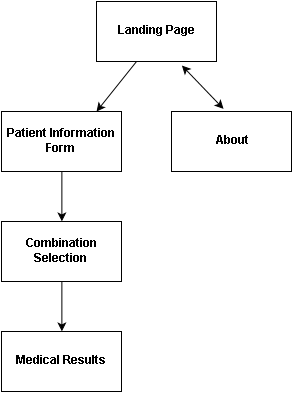
\includegraphics{navflow.png}
  \caption{Diagram of HIV Regimen Generator UI Navigation Flow}
  \label{fig:Diagram of HIV Regimen Generator UI Navigation Flow}
\end{figure}

\subsection{Landing Page}
The landing page is the “home” page of the website, where the: title, logo, and the navbar containing other valuable links will be displayed. From this page, the user will be able to begin using our application by clicking the “Start Here” button found in the middle of the page.

\begin{figure}[!h]
  \centering
  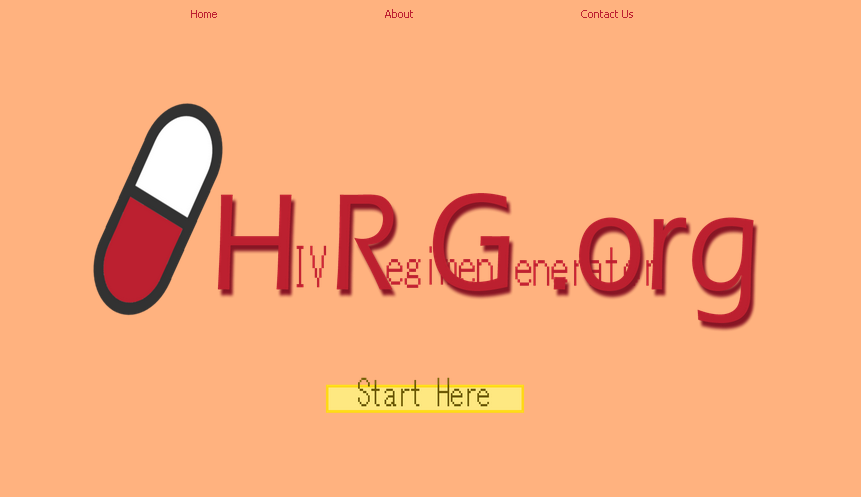
\includegraphics[width=\linewidth]{landing.png}
  \caption{Screen image of Landing page}
  \label{fig:landing}
\end{figure}

\subsection{About}
The “About” link in the navigation bar will redirect the user to the about page. It will be used to inform users about the purpose and functionality of the web application. The about page will provide necessary background information, as well as detailed instructions on how to correctly fill the patient form and select a compatible regimen.

\subsection{Patient Information Form}
The purpose of the Patient information form is to gather relevant information from the doctor or user about the patient that will be using the generated medical regimen. The information required is: age, height, weight, tanner stage, HLA status, medical issues, resistance to medications, types of medication the patient can take and relevant allergies. The BSA, which is the body surface area used to calculate safe doses of a medication, can also be calculated on this page with the data provided by the client. This is the page where the data is stored before the database is called to retrieve possible medication combinations for the patient.

\begin{figure}[H]
  \centering
  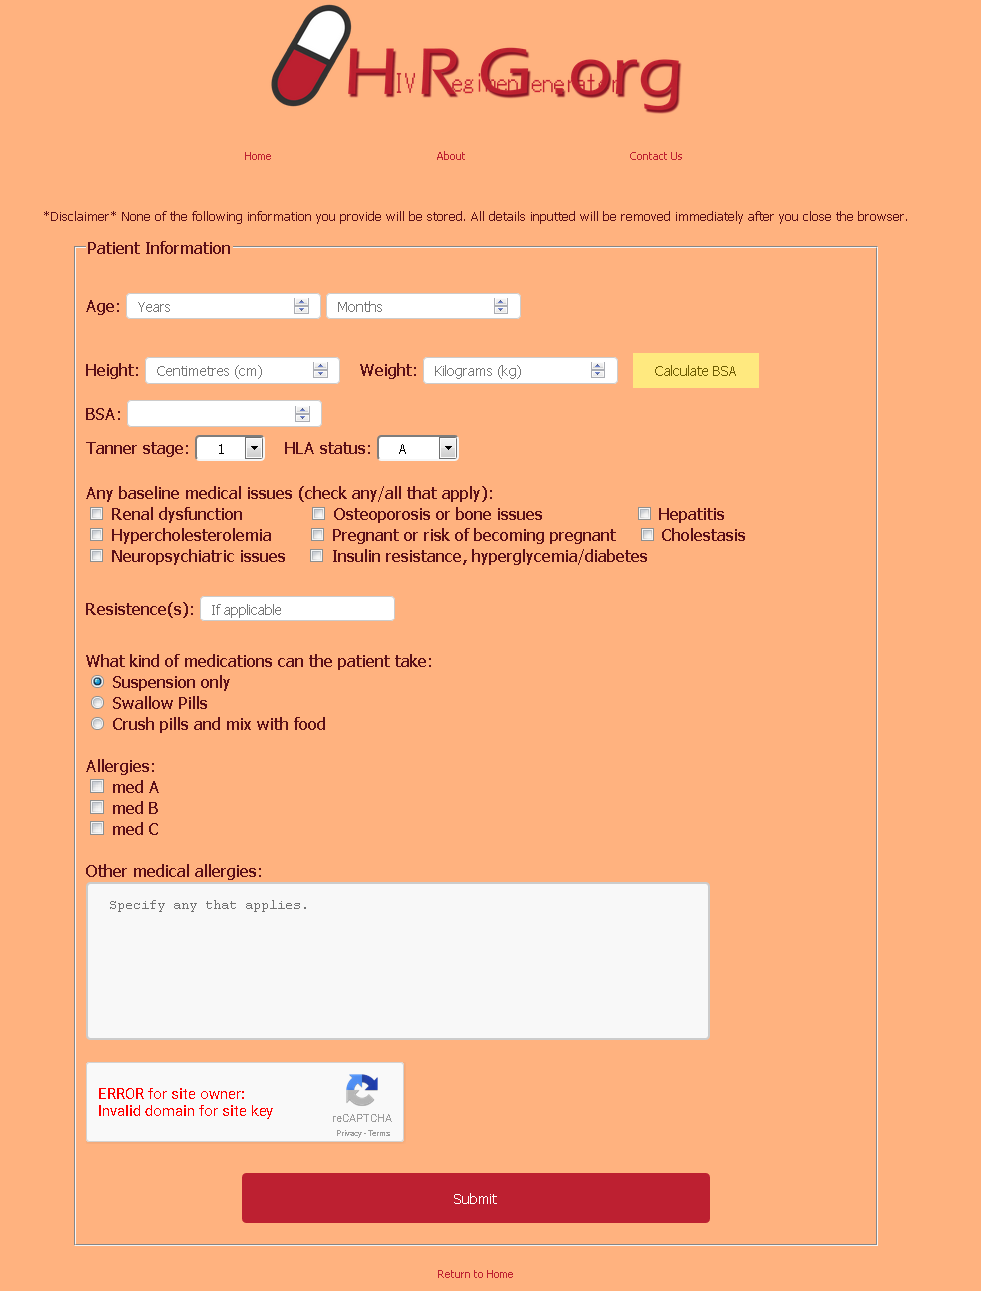
\includegraphics[width=\linewidth]{form1.png}
 \caption{Screen image of Patient Information page}
  \label{fig:form1}
\end{figure}

\subsection{Combination Selection}
Once the patient's information is filled out on the form page, our algorithm will generate a list of compatible medical regimen to be administered to the patient in the form of radio buttons on the combination selection page. Each of the medications will be grouped in combinations of two or three medications to differentiate between possible regimens. The user will be prompted to click on the radio button of the single combination of medications that they would like to use and the continue button will be clicked to confirm.

\begin{figure}[H]
  \centering
  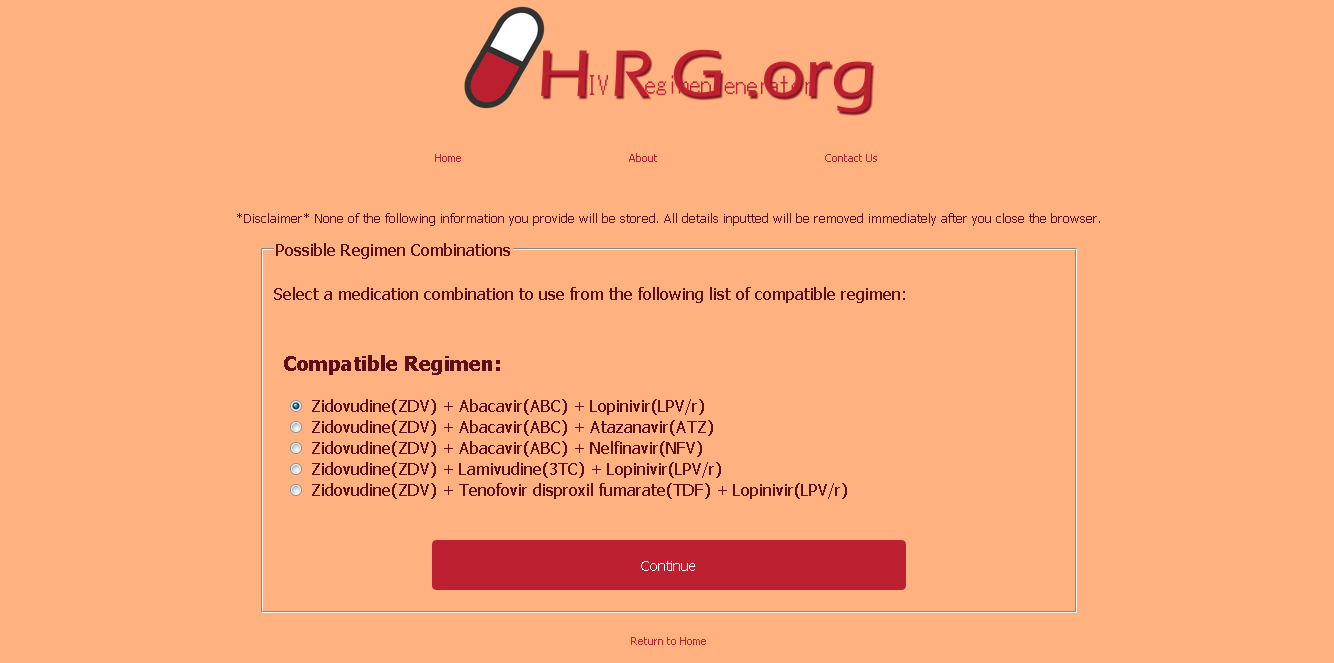
\includegraphics[width=\linewidth]{combo.png}
  \caption{Screen image of Combination Selection page}
  \label{fig:combo}
\end{figure}

\subsection{Medical Results}
The medical results page will follow the combination selection page. It gives the user a more detailed description of each of the medications present in the selected regimen. It will also include valuable information such as a suggested dosage and potential side effects of long term use. The user will have the option to print out this page through a button found on the bottom of the page.

\begin{figure}[H]
  \centering
  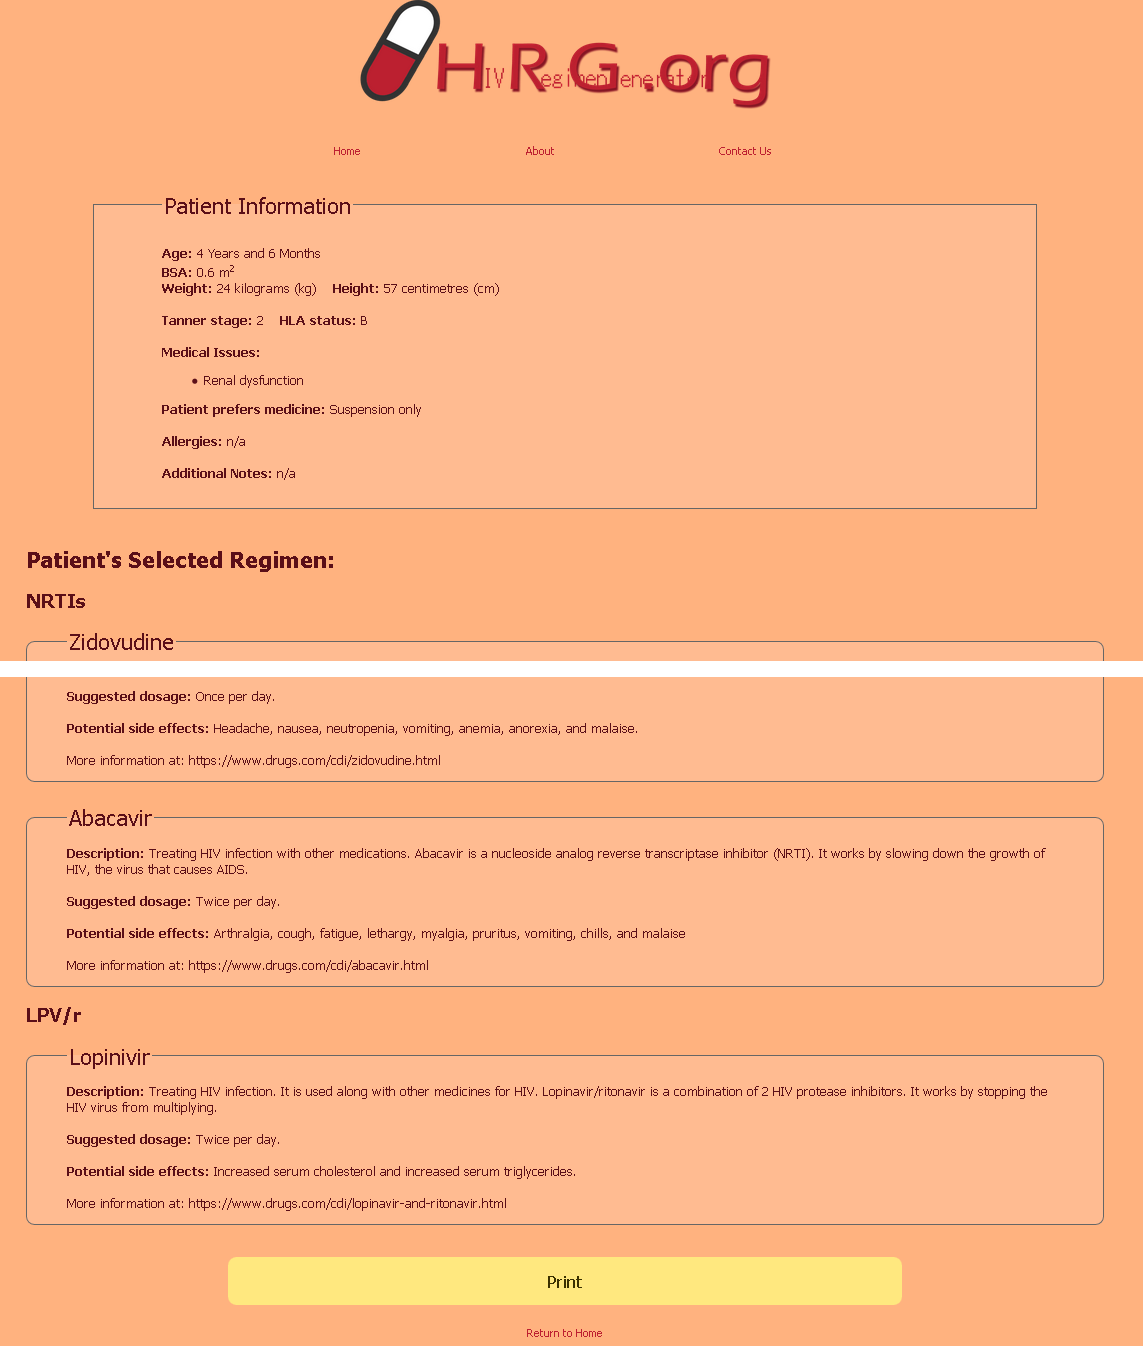
\includegraphics[width=\linewidth]{results1.png}
  \caption{Screen image of Medical Results page}
  \label{fig:results1}
\end{figure}

\section{Module Decomposition}

\subsection{Patient Information Form}
The algorithm for our web application will be tested first, as it is the most important feature of the webpage. User experience and UI testing will commence after this.
\begin{itemize}
\item Stores any relevant patient information with the information given by the client
\item \textbf{age(ageID)} - stores the age of the patient
\item \textbf{height(heightID)} - stores the height of the patient
\item \textbf{weight(weightID)} - stores the weight of the patient
\item \textbf{bsa(bsaID)} - stores the BSA that is calculated using the height and weight
\item \textbf{tannerStage(tannerID)} - stores the Tanner stage of the patient
\item \textbf{hlaStatus(hlaID)} - stores the HLA status of the patient
\item \textbf{medicalIssues(issuesID)} - stores any medical issues the patient may have
\item \textbf{resistance(resistanceID)} - stores any medication resistance the patient may have
\item \textbf{medications(medicationsID)} - stores the types of medication the patient can take
\item \textbf{allergies(allergiesID)} - stores any allergies the patient may have
\end{itemize}

\subsection{Data retrieval from database}
\begin{itemize}
\item Creates different combinations of medicine for the user to take
\item \textbf{checkage(ageID)} - checks if the medication is compatible with the age of the patient
\item \textbf{checkbsa(bsaID)} - checks if the medication is compatible with the BSA of the patient
\item \textbf{checktannerStage(tannerID)} - checks if the medication is compatible with the Tanner stage of the patient
\item \textbf{checkhlaStatus(hlaID)} - checks if the medication is compatible with the HLA status of the patient
\item \textbf{checkmedicalIssues(issuesID)} - checks if the medication is compatible with the medical issues of the patient
\item \textbf{checkresistance(resistanceID)} - checks if the medication is compatible with the resistance of the patient
\item \textbf{checkmedications(medicationsID)} - checks if the medication is compatible with the type of medications that the patient can take
\item \textbf{checkallergies(allergiesID)} - checks if the medication is compatible with the allergies of the patient
\item \textbf{combo1()} - creates the first combination (assigns any ARVS to arvList that are used in the combo so that another combination does not reuse them)
\item \textbf{combo2(arvList)} - creates the first combination (assigns any ARVS to arvList that are used in the combo so that another combination does not reuse them)
\item \textbf{combo3(arvList)} - creates the first combination of ARVS for the patient
\item \textbf{combo(comboID)} - identifies which combination has been selected using the comboID as an integer from 1 to 3
\end{itemize}


\subsection{Drug information results page}
\begin{itemize}
\item Displays all relevant information to the client
\item\textbf{generateResults(comboID,ageID,weightID,heightID,bsaID,tannerID,hlaID,issuesID,resistanceID,medicationsID,allergiesID)} - creates the page using any important information
\end{itemize}

\section{Relational Database Structure}

\subsection{ER Diagram}
\begin{figure}[H]
  \centering
  \includegraphics[width=\linewidth]{ERdiagram.png}
  \caption{ER-Diagram}
  \label{fig:er}
\end{figure}

\subsection{Table Descriptions}
\begin{itemize}
\item \textbf{medication} - stores information about the medication such as its type and description of use (id, type, description, name)
\item \textbf{patientRequirements} - stores requirements that the patient must possess in order to use the medication (id,ageMin, ageMax, weightMin, weightMax, tannerStage, medicalIssue, BSA, HLA, resistance, allergies)

\item \textbf{limitations} - contains diseases and dysfunctions that may limit the patient from using the drug (id, renalDysfunction, osteoporosis, hepatitis, hypercholesterolemia, pregnancy, cholestasis, neuropsychiatric, insulinResistance, hyperglycemia, diabetes)

\item \textbf{dosage} - contains possible dosages that may be taken for this medication (id, amount, timesPerDay)
\item \textbf{sideEffects} - contains description of the side effects that may result from medication use (id, sideEffectList)
\end{itemize}

\section{Communication Protocol}
This application uses Hypertext Transfer Protocol (HTTP) to communicate between web page and server. HTTP is an application protocol for distributed, collaborative, hypermedia information systems.


\section{Development Details}

\subsection{Languages of implementation}
\begin{itemize}
\item HTML
\item CSS
\item PHP
\item JavaScript
\item SQL
\end{itemize}

\subsection{Supporting technology}
\begin{itemize}
\item Apache server
\item MySQL
\end{itemize}

\section{References}
[1] Don Norman. The Design of Everyday Things - Revised and Expanded Edition. Basic
Books, New York, 10-131, 2013.

\end{document}